\section{Pregunta N$^{\circ}$8\qquad Carlos Alonso Aznarán Laos}

\begin{frame}
    \begin{enumerate}\setcounter{enumi}{7}
        \item

              Evalúe la función
              \begin{math}
                  f\left(x\right)=
                  \dfrac{
                  10\ln\left(x^{2}+x+1\right)
                  }{
                  10x^{3}-20x^{2}+x-2
                  }
              \end{math}
              en siete nodos igualmente espaciados del intervalo
              $\left[-1,1\right]$.

              \begin{enumerate}[a)]
                  \item

                        Construya un spline cúbico que interpone a
                        $f$ en dichos puntos.

                  \item

                        Calcule el error
                        \begin{math}
                            e\left(x\right)=
                            f\left(x\right)-
                            s\left(x\right)
                        \end{math}.

                  \item

                        Gráfique las tres funciones.
                        ¿Qué puede decir de dichas gráficas?
              \end{enumerate}
    \end{enumerate}

    \begin{solution}
        Vamos a resolver el sistema lineal por

        \begin{figure}[ht!]
            \centering
            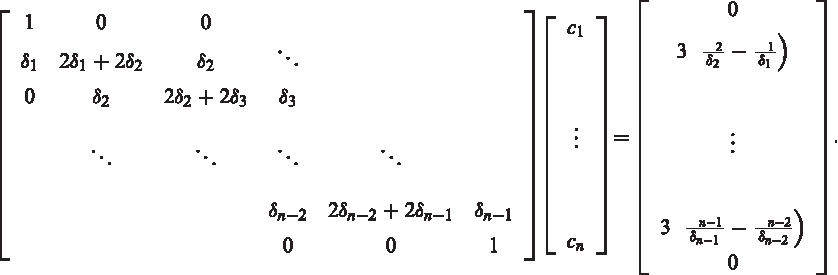
\includegraphics[width=.65\paperwidth]{system}
        \end{figure}
    \end{solution}
\end{frame}

\begin{frame}
    \begin{solution}
        \begin{figure}[ht!]
            \centering
            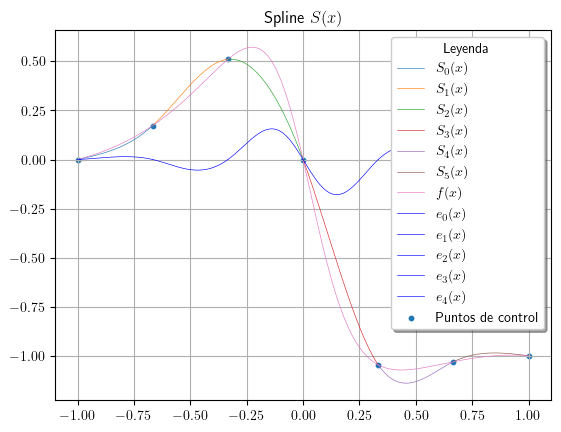
\includegraphics[width=.65\paperwidth]{8}
        \end{figure}
    \end{solution}
\end{frame}
